\chapter[supplementary material: model-agnostic out-of-distribution detection using combined statistical tests]{Supplementary material: Model-Agnostic Out-of-Distribution Detection Using Combined Statistical Tests}
\label{app:supplementary-modelagnostic}
\ifthenelse{\equal{\skipappendices}{true}}{}{

\section{Crude approximation of the Fisher information}
\label{appendix_modelagnostic:cheap}

The Fisher information is defined as:
\begin{equation}
    I({\theta}) =  \mathbb{E}_{x \sim p_\theta}[\nabla \log {p_\theta}(x) \nabla  \log {p_\theta}(x) ^T].
\end{equation}

A crude diagonal approximation can be computed by simply estimating the diagonal of $I({\theta})$ and setting all off-diagonal elements to zero. Such diagonal approximations have been used in machine learning for decades: for instance, \textcite[Section 3.12.2]{lecun_modeles_1987} used a similar approximation of the Hessian matrix, and called it ``outrageously simplifying". Much more complex approximations have been derived, although diagonal approximations have been consistently used (e.g. by \citealp{kirkpatrick_overcoming_2017}, who used essentially the same approximation in a supervised context), and are linked to several adaptive optimisation techniques like Adam \parencite{kingma_adam_2015} or RMSProp \parencite{tieleman_lecture_2012}. A good discussion on these issues is provided in Martens's \citeyearpar{martens_new_2020} recent review.

The approximation we used in the paper works as follows:
\begin{itemize}
    %\item We first sample $x_1,...,x_T\sim p_\theta $ according to the learned generative model (which will be relatively cheap in most cases).
    \item By using the training examples $x_1,...,x_T$, we form the estimate
    $$ {D}_T({\theta}) = \frac{1}{T} \sum_{t=1}^T \textup{diag}(\nabla \log {p_\theta}(x_t)^2),  $$
    where the square in $\nabla \log p_\theta(x_t)^2$ is computed elementwise.
    \item While we could directly use ${D}_T({\theta})$ as an estimate. A slightly more refined approach is to slightly regularise $D_T({\theta})$. Following \textcite{martens_new_2020}, our final estimate of the Fisher information matrix is
    \begin{equation}
    	\hat{I}_T({\theta}) = (D_T({\theta}) + \varepsilon)^\xi,
    \end{equation}
    with all operations performed elementwise. The diagonal matrix $\hat{I}_T({\theta})$ is then easy to invert and can be used to compute our statistics.
\end{itemize}


\paragraph{How to choose $\varepsilon$ and $\xi$?} The Adam optimizer uses a similar estimate, with default hyperparameters $\varepsilon = 10^{-8}$ and $\xi = 1$. As argued by \textcite{martens_new_2020}, it can be interesting to use $\xi <1$  in order to diminish the influence of extreme values of $D_T({\theta})$. In particular, \textcite{martens_new_2020} suggests taking $\xi = 0.75$. When $\xi \longrightarrow 0$, then $\hat{I}_T({\theta})$ will approach the identity matrix. We tested the two settings by using a PixelCNN++ trained on CIFAR. Results are shown in \cref{tab_modelagnostic:martens}. In terms of OOD detection, it seems that using $\varepsilon = 10^{-8}$ and $\xi = 1$ is slightly better. All results presented in the paper and in the supplementary material are computed by using $\varepsilon = 10^{-8}$ and $\xi = 1$.



\paragraph{A few notes on the computation of $D_T({\theta})$} While it seems more sensible to use samples $x_1,...,x_m\sim p_\theta $ from the model, we decided to simply reuse the training data $x_1,...,x_T $ instead. There are two computational advantages to this. The first one is that sampling many data points can be expensive (in particular for deep autoregressive models à la PixelCNN). The second advantage is that, if we wish to compute a MMD statistic, such as the MMD with the Fisher kernel or the MMD typicality (that require the average of gradient or the average log-likelihood over the training), computing the average of the square of the gradient costs very little. One can just do a single loop over the data, and use the usual formulas for online estimation of a mean, see \cref{alg_modelagnostic:algo_description}.


\paragraph{Do we really need to approximate the diagonal of $I({\theta})$?} 
Another possibility is to just use the identity matrix as FIM instead of of approximating the diagonal through the procedure explained above. In our experiments (see \cref{tab_modelagnostic:mmd} and \cref{tab_modelagnostic:mmd_pair2}), we can see that sometimes using the identity matrix seems to work equally well or a bit better for some models trained on FashionMNIST and CIFAR10. However, when we train on SVHN or MNIST, there are a cases where the statistic that is using the identity matrix as approximation fails, sometimes being worse than random chance. In those setting, using the diagonal approximation leads to way better results. Therefore, considering a test statistic that uses the diagonal approximation of the FIM is more robust for OOD detection.


\begin{table*}[tb]
    \centering
    \caption[AUROC$\uparrow$ for single-sample OOD detection comparing two different estimates of the Fisher information matrix]{AUROC$\uparrow$ for single-sample OOD detection. Comparison between two different estimates of the Fisher information matrix. For ($\ddagger$) we used the Adam parameter choice, i.e.\@ $\varepsilon = 10^{-8}$ and $\xi = 1$. For ($\mathsection$), instead, we used  $\varepsilon = 10^{-8}$ and $\xi = 0.75$, as suggested by \textcite{martens_new_2020}. As a result, we have that using Adam parameters choice is slightly better for our task.}
    \resizebox*{\textwidth}{!}{
    \small
    \begin{tabular}{ccccc}
        \toprule
        &\multicolumn{4}{c}{\textsc{CIFAR10 (in) / SVHN (out)}}\\
        \cmidrule{2-5}
        \textsc{models}  & \textcolor{blue}{\textsc{MMD diagonal}} &  \textcolor{blue}{\textsc{Typicality}} & \textcolor{blue}{\textsc{Score stat}} & \textcolor{red}{\textsc{Fisher's method}} \\
        \midrule
        \textsc{PixelCNN++} (model2) ($\ddagger$) & 0.7070 & 0.6498  &  0.7067 & 0.7300\\
        \textsc{PixelCNN++} (model2) ($\mathsection$) & 0.6881 &  0.6498  & 0.6878 & 0.7176\\
        \bottomrule
        \vspace{-0.2cm}\\
        ($\ddagger$) With $\varepsilon = 10^{-8}$ and $\xi = 1$ \\
        \hspace{0.4cm}($\mathsection$) With $\varepsilon = 10^{-8}$ and $\xi = 0.75$
    \end{tabular}
    \label{tab_modelagnostic:martens}
    }
\end{table*}



\section{The Mahalanobis score as MMD}
\label{appendix_modelagnostic:mahalanobis}

\textcite{lee_simple_2018} introduced a simple metric to perform OOD detection with a trained deep classifier. The key idea is to train a simple generative model (linear discriminant analysis) in the feature space of the classifier. Let $y$ denote the labels, and $z = f(x)$ the data in feature space. In the simplest case, $f$ is just the trained deep net devoid of the last softmax layer. The linear discriminant analysis model is
\begin{equation}
    y \sim \textup{Cat}(\pi), \; \; z | y \sim \mathcal{N}(\mu_y, \Sigma),
\end{equation}
where $\mu_1,...,\mu_K$ are class-dependent means, $\Sigma$ a common covariance matrix, and $\pi_1,...,\pi_K$ are the class proportions, estimated by maximum-likelihood. The \emph{Mahalanobis score} is then
\begin{equation}
    M(x) = \max_{k \in \{1,...,K \}} - (z - \mu_k)^T \Sigma^{-1} (z - \mu_k),
\end{equation}
which may be rewritten
\begin{equation}
    M(x) = \max_{k \in \{1,...,K \}} p(z|k),
\end{equation}
under the assumption of equal class proportions (i.e.\@ $\pi_1 = ... = \pi_K = 1/K$).

We show here that it is possible to re-interpret this score as a MMD score with a certain Fisher kernel. 
The generative model induced on $z$ by linear disciminant analysis is a Gaussian mixture:
\begin{equation}
    p_{\pi, \mu , \Sigma }(z) = \sum_{k=1}^K \pi_k \mathcal{N}(z | \mu_k, \Sigma).
\end{equation}
If we want a powerful deep kernel, it seems somewhat natural to consider the Fisher kernel associated with this generative model. The most important part of this mixture model are arguably the class-specific means (indeed, the model has been trained to discriminate the classes as well as possible). Therefore, we will only include these means in the Fisher kernel, and look at
\begin{equation}
	\Phi_\textup{Fisher} (x) = I(\mu)^{-1/2} \nabla_\mu  \log p_{\pi, \mu , \Sigma }(z),
\end{equation}
assuming that $\pi$ and $\Sigma$ are fixed at their maximum likelihood estimates. Similar mixture-based Fisher kernels have been very popular in the past, and were actually a key element of state-of-the art classification models on Imagenet before deep nets won the competition \parencite{perronnin_improving_2010}. Our idea is to re-use ideas introduced by this computer vision litterature. Under the assumption that the Gaussian clusters are well-separated, \textcite{tanaka_fisher_2013}, extending an earlier analysis of \textcite[Appendix A]{sanchez_image_2013}, showed that
\begin{equation}
	[\Phi_\textup{Fisher} (x)]_{\mu_k} \approx \sqrt{\frac{p(z|k)}{\pi_k }}  \Sigma^{-1/2} (z - \mu_k).
\end{equation}
Now, using the fact that the expected value of the score is approximatively zero, we can write that
\begin{equation}
    \textup{MMD}_{\Phi_\textup{Fisher}}^2 \approx \sum_{k=1}^K  \parallel [\Phi_\textup{Fisher} (x)]_{\mu_k} ||_2^2 \approx \sum_{k=1}^K \frac{p(z|k)}{\pi_k} (z - \mu_k)^T \Sigma^{-1} (z - \mu_k).
\end{equation}



Using again the fact that the clusters are well-separated, we may say that $z|k$ is approximatively a point mass at the most probable label,  i.e.\@ that $p(z|k) \approx \delta_k^{\text{argmax}_c p(z|c)}$. This leads to the approximation 
\begin{equation}
    \textup{MMD}_{\Phi_\textup{Fisher}}^2 \approx \max_{k \in \{1,...,K\}} \frac{1}{\pi_k} (z - \mu_k)^T \Sigma^{-1} (z - \mu_k).
\end{equation}
Finally, assuming that the class proportions are equal leads to the equivalence of $\textup{MMD}_{\Phi_\textup{Fisher}}$ and the Mahalanobis score.




\section{More Information on the experimental setup}

\subsection{A bit more background}
The three considered DGMs are both parametrized by neural networks but they differ in the way they model the data distribution of interest. Assume we are interested in approximating a target distribution $p^*(\mathbf{x})$, for example a distribution of natural images, as it is done when using CIFAR10. PixelCNN++ is an autoregressive model and it models $p^*(\mathbf{x})$ as a product of conditional distribution over the variables, i.e.\@ $p(\mathbf{x}) = p(x_1) \prod_{d=2}^D p(x_d \mid \mathbf{x}_{<d})$, where $\mathbf{x}_{<d} = [x_1, \dots, x_{d-1}]^T$. Glow is a normalizing flow model and it approximate $p^*(\mathbf{x})$ by using a sequence of bijiective transformations starting from a simple distribution, also called base distribution. If we use only a single invertible transformation $f$, the normalizing  flow is defined as $\mathbf{x} = f(\mathbf{z})$, where $\mathbf{z} \sim p_{Z}(\mathbf{z})$, and $p_{X}(\mathbf{x}) = p_{Z}(\mathbf{z})|\det J_f(\mathbf{z}) |^{-1}$, where we used the change of variable formula. For these two types of model we have a tractable likelihood that can be used to optimize the model parameters. The Variational Autoencoder (VAE), instead, is a framework to model the data with a latent variable model, i.e.\@ $p(\mathbf{x}, \mathbf{z}) = p(\mathbf{x} \mid \mathbf{z}) p(\mathbf{z})$, where $\mathbf{x}$ is the observed input data and $\mathbf{z}$ is a stochastic latent variable and the prior distribution $p(\mathbf{z})$ is usually a standard Normal. Since the posterior $p(\mathbf{z}\mid\mathbf{x})$ is not tractable, a variational distribution $q_{\phi}(\mathbf{z}\mid\mathbf{x})$ is used as an approximation. Due to the intractability of the posterior, we cannot directly optimize the likelihood of the model, but instead the model parameters are optimized by maximizing the evidence lower bound (ELBO): $\log p_{\theta}(\mathbf{x}) \geq \mathbb{E}_{q_{\phi}(\mathbf{z}\mid \mathbf{x})} \left[ \log \frac{p(\mathbf{x}, \mathbf{z})}{q_{\phi}(\mathbf{z}\mid \mathbf{x})} \right] \equiv \mathcal{L} $. In this work we are considering an Hierarchical VAE (HVAE) with bottom-up inference as done in \parencite{havtorn_hierarchical_2021}. This is an extension of the VAE framework that consider an hierarchy of $L$ latent variables $\mathbf{z} = \mathbf{z}_1,\dots, \mathbf{z}_L$. The bottom-up inference is defined as $q_{\phi}(\mathbf{z}\mid \mathbf{x}) = q_{\phi}(\mathbf{z}_1\mid \mathbf{x})\prod_{i=2}^L q_{\theta}(\mathbf{z}_i \mid \mathbf{z}_{i-1})$, while the generative path is top-down, meaning $p_{\theta}(\mathbf{x}\mid \mathbf{z}) = p(\mathbf{x}\mid \mathbf{z}_1)p_{\theta}(\mathbf{z}_1\mid \mathbf{z}_2)\cdots p_{\theta}(\mathbf{z}_{L-1}\mid \mathbf{z}_L)$. This is still trained by maximizing the ELBO. For a more in-depth explanation of these models we refer to their papers.

\subsection{Generative model details}
We will briefly describe the different model architectures and training procedures used in this paper. Since most of the models are taken from public code repositories and related papers, we will mostly invite the reader to have a look at the cited paper for a more in-depth description of the training details.
For MNIST, CIFAR10, and FashionMNIST we used 3000 examples from the test set as validation set. For SVHN, instead, we used 6032 datapoints from the test set as validation, leaving the remaining 20000 examples as test set. In \cref{tab_modelagnostic:log_like}, we reported test log-likelihood of the models used in this paper. 

\paragraph{PixelCNN++} For PixelCNN++ we used the code available in this repository\footnote{\href{https://github.com/pclucas14/pixel-cnn-pp}{\texttt{https://github.com/pclucas14/pixel-cnn-pp}}}. For the greyscale images, we used one residual block per stage with 32 filters and 5 logistic components in the discretized mixture of logistics. For natural images, instead, we used 5 residual blocks per stage with 160 filters and 10 components in the mixture. We trained all the models using Adam optimizer.

\paragraph{Glow} For training Glow models we follow \textcite{kirichenko_why_2020} and their repository\footnote{\href{https://github.com/PolinaKirichenko/flows_ood}{\texttt{https://github.com/PolinaKirichenko/flows\_ood}}}. They closely follow \textcite{nalisnick_deep_2019} and \parencite{kingma_glow_2018} implementation for multi-scale Glow, where a scale is defined as the sequence of actorm, invertible $1\times1$ convolution and coupling layers. While \textcite{kirichenko_why_2020} only considers the RMSProp optimizer, we trained two different models, one using RMSProp and one using Adam with batch-size 32. For the greyscale dataset our Glow is made up of 2 scales with 16 coupling layers, and a 3-layers highway network with 200 hidden units is used to predict the scale and shift parameters. For CIFAR10 and SVHN, instead, we used 3 scales with 8 coupling layers, and 400 hidden units for the 3-layers highway network. %Since training flow-based models is a bit unstable, in some cases we had to restart the training when the training failed. 
For a more in-depth description, we refer to the codebase and the Appendix C of \textcite{kirichenko_why_2020}.

\paragraph{Hierarchical VAE} We follow \parencite{havtorn_hierarchical_2021} for both model architecture design and training choices for our hierarchical VAEs. We used their open-sourced repository\footnote{\href{https://github.com/JakobHavtorn/hvae-oodd}{\texttt{https://github.com/JakobHavtorn/hvae-oodd}}}. As mentioned in the paper, the HVAE model we used has a bottom-up inference path and a top-down generative path. We trained each model for 1000 epochs using Adam optimizer with learning rate $3e-4$ and a batch-size of $128$. All models were initialized using the data-dependent initialization and they used weight-normalization \parencite{salimans_weight_2016}. In addition to that, we always consider a hierarchy of three latent variables. For greyscale images (MNIST and FashionMNIST) we used a latent dimension of $8-16-8$ for $\mathbf{z}_1, \mathbf{z}_2, \mathbf{z}_3$ respectively, while for natural images (CIFAR10 and SVHN) we used $8-16-32$. For a more in depth description of the model, we refer to Appendix B of \textcite{havtorn_hierarchical_2021}.


% table with log-likelihood (bits/dim) of the models
\begin{table*}[tb]
    \caption{Test log-likelihood (bits/dim) on MNIST, FashionMNIST, SVHN, and CIFAR10 achieved by the models used in the paper.}
    \label{tab_modelagnostic:log_like}
    \begin{subtable}{0.48\textwidth}
        \centering
        \scriptsize
        \resizebox*{1.05\textwidth}{!}{
        \begin{tabular}{cc}
            \toprule
            \multicolumn{2}{c}{\textsc{Models trained on FashionMNIST}}\\
            \midrule
            \textsc{models}  & \textcolor{black}{\textsc{Log-Likelihood (bits/dim)}}\\
            \midrule
            \textsc{PixelCNN++} (dropout) & 2.75 \\
            \textsc{PixelCNN++} (no dropout) & 2.72 \\
            \textsc{Glow} (RMSProp) &  3.04\\
            \textsc{Glow} (Adam)  & 3.02 \\
            \textsc{HVAE} ($**$) & 0.43 \\
            \bottomrule
            &   \\
            \toprule
            \multicolumn{2}{c}{\textsc{Models trained on CIFAR10}}\\
            \midrule
            \textsc{models}  & \textcolor{black}{\textsc{Log-Likelihood (bits/dim)}}\\
            \midrule
            
            \textsc{PixelCNN++} (model1)  & 2.94  \\
            \textsc{PixelCNN++} (model2)  & 2.94 \\
            \textsc{Glow} (RMSProp)   & 3.62 \\
            \textsc{Glow} (Adam)  & 3.62  \\
            \textsc{HVAE}  & 3.87 \\
            \bottomrule
            \vspace{-0.2cm}\\
            ($**$) Binarized FashionMNIST
        \end{tabular}%
        }
    \end{subtable}%
    \hspace{0.02\textwidth}
    \begin{subtable}{0.48\textwidth}
        \centering
        \scriptsize
        \resizebox*{0.95\textwidth}{!}{
        \begin{tabular}{cc}
            \toprule
            \multicolumn{2}{c}{\textsc{Models trained on MNIST}}\\
            \midrule
            \textsc{models}  & \textcolor{black}{\textsc{Log-Likelihood (bits/dim)}}\\
            \midrule
            \textsc{PixelCNN++} (dropout) & 0.90 \\
            \textsc{Glow} (RMSProp)  &  1.32 \\
            \textsc{Glow} (Adam)   & 1.30 \\
            \textsc{HVAE} ($**$)   &  0.16\\
            \bottomrule
            &   \\
            \toprule
            \multicolumn{2}{c}{\textsc{Models trained on SVHN}}\\
            \midrule
            \textsc{models}  & \textcolor{black}{\textsc{Log-Likelihood (bits/dim)}}\\
            \midrule
            \textsc{PixelCNN++} (dropout)  & 1.58 \\
            \textsc{Glow} (RMSProp)   & 2.23 \\
            \textsc{Glow} (Adam)  & 2.21  \\
            \textsc{HVAE}  & 2.38 \\
            \bottomrule
            \vspace{-0.2cm}\\
            ($**$) Binarized MNIST
        \end{tabular}%
        }
    \end{subtable}
    %\vspace*{-\baselineskip}
\end{table*}


\section{Additional results}

\subsection{Typicality test and score statistic are uncorrelated}
\label{appendix_modelagnostic:correlation}
To test if the typicality test and the score statistic are uncorrelated, we plot the two scores computed on the validation set. As can be seen from \cref{fig_modelagnostic:corralation}, we have that the two measures are not correlated as it is also highlight by the correlation coefficient.

\begin{figure}[tb]
    \centering
    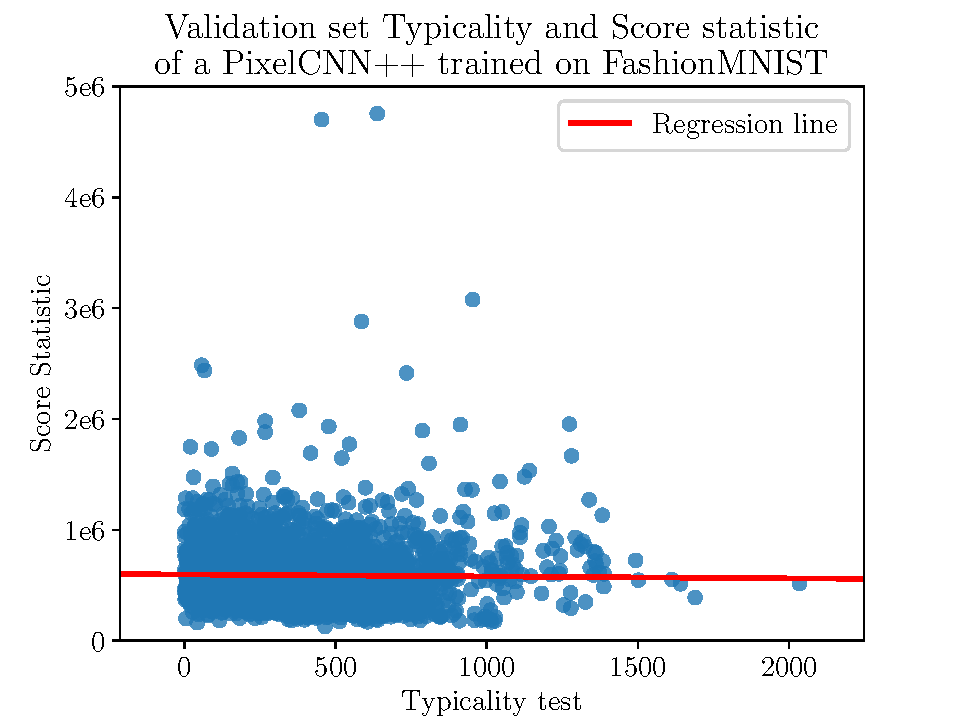
\includegraphics[scale=0.5]{graphics/paper_modelagnostic/correlation_correct_font.pdf}
    \caption[Correlation of typicality test and score statistic computed on the validation set using a PixelCNN++ trained on FashionMNIST]{Correlation of typicality test and score statistic computed on the validation set using a PixelCNN++ trained on FashionMNIST. The correlation coefficient is $-0.014$. This can also be seen by looking at the regression line, which is almost straight. }
    \label{fig_modelagnostic:corralation}
\end{figure}


\subsection{Harmonic Mean}
\label{appendix_modelagnostic:harmonic}
In the paper we mentioned that another way to combine $p$-values from different test statistics is the Harmonic mean \parencite{wilson_harmonic_2019}. This is defined as:
\begin{equation}
    \mathring{p} = \frac{\sum_{i=1}^{k} w_i}{\sum_{i=1}^{k} w_i / p_i},
\end{equation}
where $w_1,\dots,w_k$ are weights that sum up to 1. In our setting, we considered equal weights, i.e.\@ $w_i = 1 / k$. Therefore, if we simply consider two test statistics $T_1$ and $T_2$ and corresponding $p$-values $p_1$ and $p_2$, the harmonic mean $p$-values becomes:
\begin{equation}
    \mathring{p} = \frac{2 p_1 p_2}{p_1 + p_2}.
\end{equation}

As expected, this combination should work better when the statistics that we are combining are somewhat correlated. Indeed, since in our setting we have that the typicality and the score statistic are independent, we would expect this to work worse than the Fisher's combination. This is confirmed by \cref{tab_modelagnostic:all_combinations}, where we are reporting the results when combining the two statistics using the three different ways we analyzed.

\subsection{Results considering maximum-mean-discrepancy}
In \cref{sec_modelagnostic:section4}, we discussed the relationship between the maximum-mean-discrepancy with a Fisher kernel and the score statistic and the gradient norm, which depends on the choice of approximation of the Fisher information matrix we use. In \cref{tab_modelagnostic:mmd} we reported also the AUROC scores for the MMD with Fisher kernel considering both the diagonal approximation of the FIM (called \emph{MMD diagonal} in the table) and the FIM being the identity matrix (called \emph{MMD identity}). As expected, we have that the AUROC of the MMD with the diagonal approximated FIM is pretty close to the AUROC we obtained by using the score statistic. Likewise, we have that the AUROC of MMD with the identity matrix as FIM is close to the gradient norm when we trained on FashionMNIST and CIFAR10. 

So, why did we decide to use the score statistic instead of the MMD with Fisher kernel and diagonal approximation of the FIM? The main reason is Occam's razor. If we have two things that work equally well, we should keep the simplest one. In our case, we have that for computing the MMD with the Fisher kernel, we need to compute both the average gradient and the FIM using the training set. For the score statistic, instead, we just need the FIM. In addition to that, from all our experiments (see \cref{tab_modelagnostic:mmd} and \cref{tab_modelagnostic:mmd_pair2}) we do not have any evidence for one statistic working better than the other, because they are always pretty close to each other.

% \begin{table*}[]
%     \centering
%     \begin{tabular}{ |p{3.5cm}||p{1cm}|p{1cm}|p{1cm}|p{1cm}|p{1cm}|p{1cm}||p{1cm}|p{1cm}|p{1cm}|}
%     \hline
%  \multicolumn{10}{|c|}{\textbf{FashionMNIST (in) / MNIST (out)}} \\
%  \hline
%  \multicolumn{1}{|c||}{} &
%  \multicolumn{6}{|c||}{\hspace{1cm} \textbf{Single statistics}} &
% \multicolumn{3}{|c|}{\textbf{Combinations}} \\
% \hline
%         Model & $\log p(x)$ & $\left\|\nabla\right\|$ & MMD F & MMD F id &  TT & Score & FC & HM & $\text{DoSE}_{\text{KDE}}$ \\
%         \hline 
%         PixelCNN++ (dropout) &  0.0762 & 0.8709 & 0.8903 & 0.8690 & 0.8314 & 0.8822 & \textbf{0.9369} & 0.9148 & 0.8822 \\
%         \hline
%         PixelCNN++ (no drop) & 0.1048 &  0.9532 & 0.9393 & 0.9539 & 0.7575 &  0.9381 & \textbf{0.9536} & 0.9392 & 0.9382 \\
%         \hline
%         Glow (RMSProp) &  0.1970 & 0.8904 & \textbf{0.9115} &  0.8986 & 0.4807 &  0.9114 & 0.8598 & 0.8853 &  0.8901\\
%         \hline
%         Glow (Adam) & 0.1223 & 0.7705 & 0.8540 & 0.7217 & 0.6987 &  0.8745 & \textbf{0.8839} & 0.8632 & 0.8752 \\
%         \hline
%         HVAE & 0.0653 & 0.8714 & 0.9574 & 0.8726 & 0.8336 & 0.9578 & \textbf{0.9708} &  0.9569 & 0.9630  \\
%         \hline
%     \end{tabular}
%     \caption{AUROC for single-sample OOD detection}
%     \label{tab_modelagnostic:my_label}
% \end{table*}


% \begin{table*}[]
%     \centering
%     \begin{tabular}{ |p{3.5cm}||p{1cm}|p{1cm}|p{1cm}|p{1cm}|p{1cm}|p{1cm}||p{1cm}|p{1cm}|p{1cm}|}
%     \hline
%  \multicolumn{10}{|c|}{\textbf{CIFAR10 (in) / SVHN (out)}} \\
%   \hline
%  \multicolumn{1}{|c||}{} &
%  \multicolumn{6}{|c||}{\hspace{1cm} \textbf{Single statistics}} &
% \multicolumn{3}{|c|}{\textbf{Combinations}} \\
% \hline
%         Model & $\log p(x)$ & $\left\|\nabla\right\|$ & MMD F & MMD F id &  TT & Score & FC & HM & $\text{DoSE}_{\text{KDE}}$ \\
%         \hline 
%         PixelCNN++ (model1) & 0.1553 & 0.8006 & 0.6406 & 0.8126 & 0.6457 & 0.6407 & \textbf{0.6826} & 0.6667 & 0.6571 \\
%         \hline
%         PixelCNN++ (model2) & 0.1567 & 0.7923 & 0.7070 & 0.7955 & 0.6498 &  0.7067 & \textbf{0.7300} & 0.7105 & 0.7243 \\
%         \hline
%         Glow (RMSProp) &  0.0630 & 0.8585 & 0.7929 & 0.8621 & 0.8651 &  0.7940 &  \textbf{0.8683} & 0.8551 & 0.8510 \\
%         \hline
%         Glow (Adam) &  0.0627 & 0.7844 & 0.7620 &  0.7838 &  \textbf{0.8624} &  0.7655 &  \textbf{0.8613} & 0.8493 & 0.8588 \\
%         \hline
%         HVAE & 0.0455 & 0.8041 &  0.7268 & 0.7634 & \textbf{0.8845} & 0.7334 & 0.8699 &  0.8525 & 0.8245  \\
%         \hline
%     \end{tabular}
%     \caption{AUROC for single-sample OOD detection}
%     \label{tab_modelagnostic:my_label}
% \end{table*}

\begin{table*}[tb]
    %\renewcommand{\thetable}{4}
    \caption[AUROC$\uparrow$ for single-sample OOD detection comparing all single statistics with models trained on FashionMNIST (tested on MNIST) and CIFAR10 (tested on SVHN)]{AUROC$\uparrow$ for single-sample OOD detection. In this table we consider all the different single statistics we mentioned in the paper with models trained on FashionMNIST and CIFAR10. One can notice that MMD diagonal is pretty close to the score statistic and the MMD identity is close to the gradient norm, as expected (see Section 4.1 in the paper). Complementary results for models trained on MNIST and SVHN are in \cref{tab_modelagnostic:mmd_pair2}.}
    \resizebox{\textwidth}{!}{
        \scriptsize
        \begin{tabular}{ccccccc}
            \toprule
            &\multicolumn{6}{c}{\textsc{FashionMNIST (in) / MNIST (out)}}\\
            \cmidrule{2-7}
            & \multicolumn{6}{c}{\textcolor{blue}{\textsc{single statistics}}}\\
            \cmidrule{2-7}
            \textsc{models}  & \textcolor{blue}{\textsc{$\log p(x)$}} & \textcolor{blue}{\textsc{$\|\nabla \log p(x)\|_2$}} & \textcolor{blue}{\textsc{MMD diagonal}}  & \textcolor{blue}{\textsc{MMD identity}} &\textcolor{blue}{\textsc{Typicality}} & \textcolor{blue}{\textsc{Score stat}}  \\
            \midrule
            \textsc{PixelCNN++} (dropout) & 0.0762 & 0.8709 & 0.8903 & 0.8690 & 0.8314 & 0.8822 \\
            \textsc{PixelCNN++} (no dropout)  & 0.1048 &  0.9532 & 0.9393 & 0.9539 & 0.7575 &  0.9381\\
            \textsc{Glow} (RMSProp) &  0.1970 & 0.8904 & 0.9115 &  0.8986 & 0.4807 &  0.9114\\
            \textsc{Glow} (Adam)  &0.1223 & 0.7705 & 0.8540 & 0.7217 & 0.6987 &  0.8745\\
            \textsc{HVAE}  &0.0653 & 0.8714 & 0.9574 & 0.8726 & 0.8336 & 0.9578 \\
            \bottomrule
            & & & & & & \\
            \toprule
            &\multicolumn{6}{c}{\textsc{CIFAR10 (in) / SVHN (out)}}\\
            \cmidrule{2-7}
            & \multicolumn{6}{c}{\textcolor{blue}{\textsc{single statistics}}}\\
            \cmidrule{2-7}
            \textsc{models}  & \textcolor{blue}{\textsc{$\log p(x)$}} & \textcolor{blue}{\textsc{$\|\nabla \log p(x)\|_2$}} & \textcolor{blue}{\textsc{MMD diagonal}}  & \textcolor{blue}{\textsc{MMD identity}} &\textcolor{blue}{\textsc{Typicality}} & \textcolor{blue}{\textsc{Score stat}}  \\
            \midrule
        
            \textsc{PixelCNN++} (model1)  & 0.1553 & 0.8006 & 0.6406 & 0.8126 & 0.6457 & 0.6407 \\
            \textsc{PixelCNN++} (model2) & 0.1567 & 0.7923 & 0.7070 & 0.7955 & 0.6498 &  0.7067\\
            \textsc{Glow} (RMSProp)  & 0.0630 & 0.8585 & 0.7929 & 0.8621 & 0.8651 &  0.7940\\
            \textsc{Glow} (Adam)   & 0.0627 & 0.7844 & 0.7620 &  0.7838 &  0.8624 &  0.7655 \\
            \textsc{HVAE}  & 0.0455 & 0.8041 &  0.7268 & 0.7634 & 0.8845 & 0.7334\\
            \bottomrule
        \end{tabular}
        \label{tab_modelagnostic:mmd}
    }
    % \vspace*{-0.85\baselineskip}
\end{table*}


\begin{table*}[tb]
    \centering
    %\renewcommand{\thetable}{4}
    \caption[AUROC$\uparrow$ for single-sample OOD detection comparing three methods of combining different statistics with models trained on FashionMNIST (tested on MNIST) and CIFAR10 (tested on SVHN).]{AUROC$\uparrow$ for single-sample OOD detection. Comparison between the three methods we mentioned to combine different statistics. Since the typicality and the score statistic are not correlated, we have that the Fisher's method is mostly working better than the other two methods.}
        \scriptsize
        \begin{tabular}{cccc}
            \toprule
            &\multicolumn{3}{c}{\textsc{FashionMNIST (in) / MNIST (out)}}\\
            \cmidrule{2-4}
            & \multicolumn{3}{c}{\textcolor{red}{\textsc{combinations}}}\\
            \cmidrule{2-4}
            \textsc{models}  & \textcolor{red}{\textsc{Fisher's method}} & \textcolor{red}{\textsc{Harmonic mean}} &  \textcolor{red}{\textsc{DoSE$_{\textup{KDE}}$}}  \\
            \midrule
            \textsc{PixelCNN++} (dropout) & 0.9369 & 0.9148 & 0.8822 \\
            \textsc{PixelCNN++} (no dropout)  & 0.9536 & 0.9392 & 0.9382\\
            \textsc{Glow} (RMSProp) &  0.8598 & 0.8853 &  0.8901\\
            \textsc{Glow} (Adam)  & 0.8839 & 0.8632 & 0.8752\\
            \textsc{HVAE}  & 0.9708 &  0.9569 & 0.9630\\
            \bottomrule
            & & &  \\
            \toprule
            & \multicolumn{3}{c}{\textsc{CIFAR10 (in) / SVHN (out)}}\\
            \cmidrule{2-4}
            & \multicolumn{3}{c}{\textcolor{red}{\textsc{combinations}}}\\
            \cmidrule{2-4}
            \textsc{models}  & \textcolor{red}{\textsc{Fisher's method}} & \textcolor{red}{\textsc{Harmonic mean}} &  \textcolor{red}{\textsc{DoSE$_{\textup{KDE}}$}}  \\
            \midrule
        
            \textsc{PixelCNN++} (model1)  & 0.6826 & 0.6667 & 0.6571  \\
            \textsc{PixelCNN++} (model2) & 0.7300 & 0.7105 & 0.7243 \\
            \textsc{Glow} (RMSProp)  &  0.8683 & 0.8551 & 0.8510\\
            \textsc{Glow} (Adam) & 0.8613 & 0.8493 & 0.8588  \\
            \textsc{HVAE}  & 0.8699 &  0.8525 & 0.8245 \\
            \bottomrule
        \end{tabular}
        \label{tab_modelagnostic:all_combinations}
    % \vspace*{-\baselineskip}
\end{table*}

\subsection{Variability within the same model in different checkpoints}
\label{appendix_modelagnostic:checkpoints}
As mentioned in the paper, we noticed that all statistics depend on choices we made about our model and the training procedure, such as deciding between Adam or RMSProp, or between using dropout or not. In addition to that, we find out that they can differ also within the same model at different checkpoints that obtain almost the same log-likelihood. Here we consider two Glow models, one trained with Adam and one using RMSProp on CIFAR10. For both, we consider two checkpoints that achieve the same test log-likelihood. Those trained with Adam get a log-likelihood of $3.63$ bits/dim, while the ones trained with RMSProp get $3.62$ bits/dim. Results are shown in \cref{tab_modelagnostic:variability}. It can be noticed, that although the models are similar in terms of test bits/dim the statistics vary a lot, mostly when training with RMSProp.

\begin{table*}[tb]
    \centering
    %\renewcommand{\thetable}{4}
    \caption[AUROC$\uparrow$ for single-sample OOD detection comparing two different Glow models on single and combined statistics.]{AUROC$\uparrow$ for single-sample OOD detection. In this table we are comparing two different Glow models trained on CIFAR10 by considering two different checkpoints with almost the same test log-likelihood. We can see that both statistics vary a bit.}
        \scriptsize
        \begin{tabular}{ccccc}
            \toprule
            &\multicolumn{4}{c}{\textsc{CIFAR10 (in) / SVHN (out)}}\\
            \cmidrule{2-5}
            & \multicolumn{2}{c}{\textcolor{blue}{\textsc{single statistics}}} & \multicolumn{2}{c}{\textcolor{red}{\textsc{combination}}}\\
            \cmidrule(r){2-3}\cmidrule(l){4-5}
            \textsc{models}  &  \textcolor{blue}{\textsc{Typicality}} & \textcolor{blue}{\textsc{Score stat}} & \textcolor{red}{\textsc{Fisher's method}} & \textcolor{red}{\textsc{DoSE$_{\textup{KDE}}$}} \\
            \midrule
            \textsc{Glow} (RMSProp) \{\emph{check1}\} & 0.8651 &  0.7940  &  0.8683 &  0.8510\\
            \textsc{Glow} (RMSProp) \{\emph{check2}\} & 0.8532 &  0.6894  & 0.8275 & 0.7815\\
            \midrule
            \textsc{Glow} (Adam)  \{\emph{check1}\} & 0.8624 &  0.7655 & 0.8613 & 0.8588\\
            \textsc{Glow} (Adam) \{\emph{check2}\} & 0.8558 & 0.7327 & 0.8402 & 0.8303\\
            \bottomrule
        \end{tabular}
        \label{tab_modelagnostic:variability}
    % \vspace*{-\baselineskip}
\end{table*}



\subsection{Benjamini-Hochberg procedure when training on CIFAR10}
\label{appendix_modelagnostic:BH_cifar}
In the main paper we focused on the Benjamini-Hochberg procedure applied to a model trained on FashionMNIST. Although one should use a False Discovery Rate control procedure when the statistics we are using are strong, for completeness, we will present what happens when we apply the BH procedure on a model trained on CIFAR10. In \cref{fig_modelagnostic:type1_cifar}, we report the Type I error ratio and the Type II error ratio for different significance levels $\alpha$. We can see that we can actually control the FDR for $\alpha > 0.2$, and for these significance levels we are actually controlling the FDR. What is happening for $\alpha < 0.2$? We have that the procedure is only rejecting 5 hypotheses and all these hypotheses corresponds to in-distribution examples. Therefore, we have that the ratio of Type I error is still low, but we are making a lot of Type II errors because we are accepting all the examples whose hypotheses should be rejected.

%%%%%%%%%%%%%%%%%%%%%%% FIGURE
\begin{figure}[tb]
    \centering
    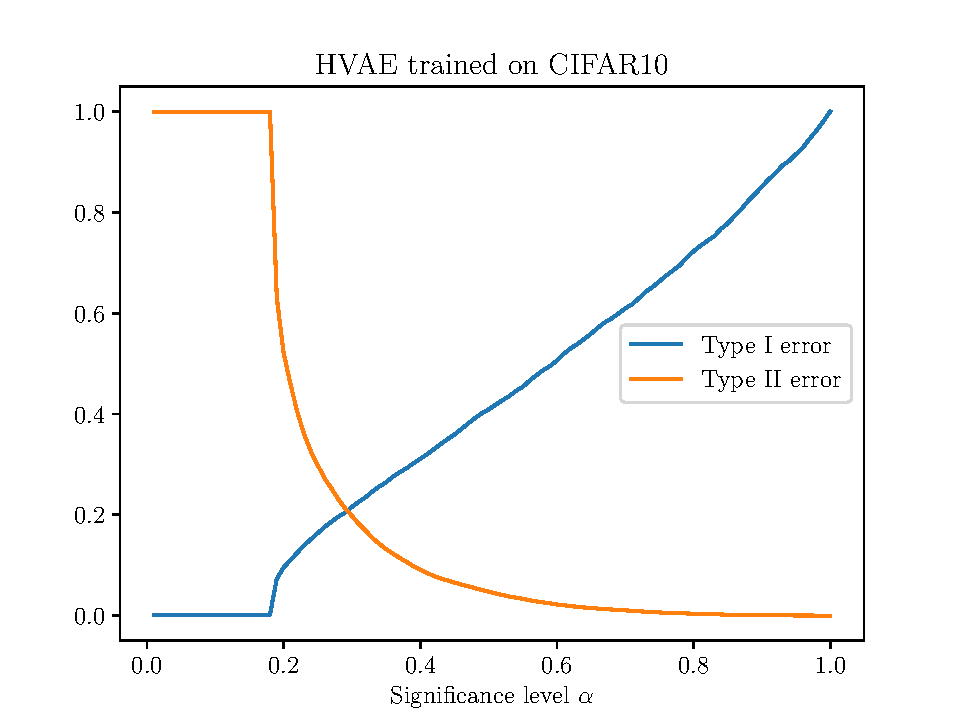
\includegraphics[scale=0.5]{graphics/paper_modelagnostic/cifar_hvae_type1_correct_font.pdf}
    \caption[Type I and Type II errors versus the significance level $\alpha$ on the combination values.]{Type I and Type II errors versus the significance level $\alpha$ on the combination values. We can control the FDR only for $\alpha > 0.2$ in this case. For $\alpha >0.2$, since we are using Benjamini-Hochberg procedure, we get that the Type I error stays below identity line.}
    \label{fig_modelagnostic:type1_cifar}
    % \vspace*{-\baselineskip}
\end{figure}     

% \subsection{False positive and False negative examples}

\subsection{Results when training on MNIST and SVHN}
\label{appendix_modelagnostic:mnist_svhn}
We also evaluated our methods in the two dataset pairs, MNIST against FashionMNIST and SVHN against CIFAR10, that are usually considered easier than the tasks presented in the main paper. For both tasks, we trained two Glow models, one trained with Adam and one trained with RMSProp, one PixelCNN++ trained with dropout and a hierarchical VAE. Results are reported in \cref{tab_modelagnostic:results_second}. We can see that almost all the statistics we considered are able to almost perfectly distinguish between the in-distribution test-set and the OOD test-set. However, we can notice that the gradient norm is failing sometimes both when we trained on CIFAR10 and when we trained on FashionMNIST. From \cref{tab_modelagnostic:mmd_pair2}, instead, it is clear that we need to approximate the diagonal of the Fisher Information Matrix because if we simply consider the identity matrix, this will also fail as the gradient norm is doing.


\begin{table*}[tb]
    \caption[AUROC$\uparrow$ for single-sample OOD detection comparing all single statistics with models trained on MNIST (tested on FashionMNIST) SVHN (tested on CIFAR10)]{AUROC$\uparrow$ for single-sample OOD detection. In this table we consider all the different single statistics we mentioned in the paper with models trained on MNIST and SVHN. In this case, it is important to notice that the gradient norm and the MMD identity sometimes fail to a different extent. Complementary results for models trained on MNIST and SVHN are in \cref{tab_modelagnostic:mmd}}
    \resizebox{\textwidth}{!}{
        \scriptsize
        \begin{tabular}{ccccccc}
            \toprule
            &\multicolumn{6}{c}{\textsc{MNIST (in) / FashionMNIST (out)}}\\
            \cmidrule{2-7}
            & \multicolumn{6}{c}{\textcolor{blue}{\textsc{single statistics}}}\\
            \cmidrule{2-7}
            \textsc{models}  & \textcolor{blue}{\textsc{$\log p(x)$}} & \textcolor{blue}{\textsc{$\|\nabla \log p(x)\|_2$}} & \textcolor{blue}{\textsc{MMD diagonal}}  & \textcolor{blue}{\textsc{MMD identity}} &\textcolor{blue}{\textsc{Typicality}} & \textcolor{blue}{\textsc{Score stat}}  \\
            \midrule
            \textsc{PixelCNN++} (dropout) ($\dagger$)  & 0.9999  & 0.8534 & 0.9993 & 0.8608 & 0.9996  & 0.9993 \\
            \textsc{Glow} (RMSProp) & 0.9997  & 0.9936  & 0.9942 & 0.6609 &  0.9991 & 0.9936\\
            \textsc{Glow} (Adam)  &0.9999 & 0.6506 & 0.9993 &  0.9124 &  0.9997 &  0.9992\\
            \textsc{HVAE}  & 0.9999 & 0.9998 &  0.9999 &  0.9999 &  0.9999  & 0.9999\\
            \bottomrule
            & & & & & & \\
            \toprule
            &\multicolumn{6}{c}{\textsc{SVHN (in) / CIFAR10 (out)}}\\
            \cmidrule{2-7}
            & \multicolumn{6}{c}{\textcolor{blue}{\textsc{single statistics}}}\\
            \cmidrule{2-7}
            \textsc{models}  & \textcolor{blue}{\textsc{$\log p(x)$}} & \textcolor{blue}{\textsc{$\|\nabla \log p(x)\|_2$}} & \textcolor{blue}{\textsc{MMD diagonal}}  & \textcolor{blue}{\textsc{MMD identity}} &\textcolor{blue}{\textsc{Typicality}} & \textcolor{blue}{\textsc{Score stat}}  \\
            \midrule
            \textsc{PixelCNN++} (dropout)  & 0.9820 & 0.2670 &   0.9543 & 0.3185 & 0.9590 & 0.9543 \\
            \textsc{Glow} (RMSProp)  &  0.9917  & 0.9180 & 0.9824 & 0.9317 & 0.9830  &  0.9823 \\
            \textsc{Glow} (Adam)   &0.9913 &  0.5658 & 0.9653 & 0.7096 & 0.9779 &  0.9641 \\
            \textsc{HVAE}  & 0.9943 &  0.1011  &  0.9865 &  0.4508 & 0.9857 &  0.9862\\
            \bottomrule
            \vspace{-0.2cm}\\
            ($\dagger$) Trained using 50000 datapoints
        \end{tabular}
        \label{tab_modelagnostic:mmd_pair2}
    }
\end{table*}


\begin{table*}[tb]
    %\renewcommand{\thetable}{4}
    \caption[AUROC$\uparrow$ for single-sample OOD detection considering single and combined statistics with models trained on MNIST (tested on FashionMNIST) SVHN (tested on CIFAR10).]{AUROC$\uparrow$ for single-sample OOD detection when training on MNIST and testing against FashionMNIST and when training on SVHN and testing against CIFAR10. As before, Fisher's method is the combination of the typicality test and the test statistic. These are also combined using DoSE. Complementary results are in \cref{tab_modelagnostic:all_combinations}.}
    \resizebox{\textwidth}{!}{
        \scriptsize
        \begin{tabular}{ccccccc}
            \toprule
            &\multicolumn{6}{c}{\textsc{MNIST (in) / FashionMNIST (out)}}\\
            \cmidrule{2-7}
            & \multicolumn{4}{c}{\textcolor{blue}{\textsc{single statistics}}} & \multicolumn{2}{c}{\textcolor{red}{\textsc{combination}}}\\
            \cmidrule(r){2-5}\cmidrule(l){6-7}
            \textsc{models}  & \textcolor{blue}{\textsc{$\log p(x)$}} & \textcolor{blue}{\textsc{$\|\nabla \log p(x)\|_2$}} & \textcolor{blue}{\textsc{Typicality}} & \textcolor{blue}{\textsc{Score stat}} & \textcolor{red}{\textsc{Fisher's method}} & \textcolor{red}{\textsc{DoSE$_{\textup{KDE}}$}} \\
            \midrule
            \textsc{PixelCNN++} (dropout) ($\dagger$)  & 0.9999  & 0.8534 & 0.9996 & 0.9993 & 0.9999  & 0.9999 \\
            \textsc{Glow} (RMSProp) & 0.9997  & 0.9936  & 0.9991 & 0.9936 &  0.9992 & 0.9994\\
            \textsc{Glow} (Adam)  &0.9999 & 0.6506 & 0.9995 &  0.9992 &  0.9998 &  0.9999\\
            \textsc{HVAE}  & 0.9999 & 0.9998 &  0.9997 &  0.9999 &  0.9999  & 0.9999\\
            \bottomrule
            & & & & & & \\
            \toprule
            &\multicolumn{6}{c}{\textsc{SVHN (in) / CIFAR10 (out)}}\\
            \cmidrule{2-7}
            & \multicolumn{4}{c}{\textcolor{blue}{\textsc{single statistics}}} & \multicolumn{2}{c}{\textcolor{red}{\textsc{combination}}}\\
            \cmidrule(r){2-5}\cmidrule(l){6-7}
            \textsc{models}  & \textcolor{blue}{\textsc{$\log p(x)$}} & \textcolor{blue}{\textsc{$\|\nabla \log p(x)\|_2$}} & \textcolor{blue}{\textsc{Typicality}} & \textcolor{blue}{\textsc{Score stat}} & \textcolor{red}{\textsc{Fisher's method}} & \textcolor{red}{\textsc{DoSE$_{\textup{KDE}}$}} \\
            \midrule
            \textsc{PixelCNN++} (dropout)  & 0.9820 & 0.2670 &  0.9590 &  0.9543 & 0.9914 & 0.9824 \\
            \textsc{Glow} (RMSProp)  &  0.9917  & 0.9180 & 0.9830 & 0.9823 & 0.9913  & 0.9913 \\
            \textsc{Glow} (Adam)   &0.9913 &  0.5658 & 0.9779 & 0.9641 & 0.9883 & 0.9863 \\
            \textsc{HVAE}  & 0.9943 &  0.1011  &  0.9857 &  0.9862 & 0.9934 &  0.9862 \\
            \bottomrule
            \vspace{-0.2cm}\\
            ($\dagger$) Trained using 50000 datapoints
        \end{tabular}    
        \label{tab_modelagnostic:results_second}
    }    
\end{table*}    


\subsection{Application of our method to Gaussian Mixture Model and Probabilistic PCA}
\label{appendix_modelagnostic:gmm_ppca}
Since the method we propose is model-agnostic, we show that it can be used for out-of-distribution detection also using two simple generative models, Gaussian Mixture Model (GMM) and Probabilistic PCA (PPCA). We consider the two pairs of datasets as before, i.e.\@ FashionMNIST vs MNIST and CIFAR10 vs SVHN. Results can be seen in \cref{tab_modelagnostic:gmm_results} and \cref{tab_modelagnostic:ppca_results}. For both GMM and PPCA trained on FashionMNIST the likelihood can be used to perform OOD detection. Indeed, in this setting, they are not assigning higher likelihood to OOD data as it is the case for DGMs. This happens instead when we fit these models on CIFAR10. However, this behaviour can be due to the fact that they are really poor generative models for this dataset. It is also surprising that when training on CIFAR10 the score statistic is failing in both models. We think that this is also due to the fact that both the GMM and the PPCA are far from being good generative models for this dataset.


\begin{table*}[tb]
    \caption[AUROC$\uparrow$ for single-sample OOD detection comparing single and combined statistics using a Gaussian mixture model (GMM) trained on FashionMNIST (tested on MNIST) and CIFAR10 (tested on SVHN).]{AUROC$\uparrow$ for single-sample OOD detection using a Gaussian mixture model (GMM). For Fisher's method we mean the combination of the typicality test and the test statistic. These are also combined using DoSE.}
    \resizebox{\textwidth}{!}{
        \scriptsize
        \begin{tabular}{ccccccc}
            \toprule
            &\multicolumn{6}{c}{\textsc{FashionMNIST (in) / MNIST (out)}}\\
            \cmidrule{2-7}
            & \multicolumn{4}{c}{\textcolor{blue}{\textsc{single statistics}}} & \multicolumn{2}{c}{\textcolor{red}{\textsc{combination}}}\\
            \cmidrule(r){2-5}\cmidrule(l){6-7}
            \textsc{components}  & \textcolor{blue}{\textsc{$\log p(x)$}} & \textcolor{blue}{\textsc{$\|\nabla \log p(x)\|_2$}} & \textcolor{blue}{\textsc{Typicality}} & \textcolor{blue}{\textsc{Score stat}} & \textcolor{red}{\textsc{Fisher's method}} & \textcolor{red}{\textsc{DoSE$_{\textup{KDE}}$}} \\
            \midrule
            \textsc{50}  & 0.6627 & 0.5514  & 0.5196 & 0.8777  & 0.7689 & 0.8152 \\
            \textsc{100}   &  0.6872 & 0.5509 & 0.5575 & 0.8742 & 0.7965 & 0.7989 \\
            \bottomrule
            &  &  &   &   &  & \\
            \toprule
            &\multicolumn{6}{c}{\textsc{CIFAR10 (in) / SVHN (out)}}\\
            \cmidrule{2-7}
            & \multicolumn{4}{c}{\textcolor{blue}{\textsc{single statistics}}} & \multicolumn{2}{c}{\textcolor{red}{\textsc{combination}}}\\
            \cmidrule(r){2-5}\cmidrule(l){6-7}
            \textsc{components}  & \textcolor{blue}{\textsc{$\log p(x)$}} & \textcolor{blue}{\textsc{$\|\nabla \log p(x)\|_2$}} & \textcolor{blue}{\textsc{Typicality}} & \textcolor{blue}{\textsc{Score stat}} & \textcolor{red}{\textsc{Fisher's method}} & \textcolor{red}{\textsc{DoSE$_{\textup{KDE}}$}} \\
            \midrule
            \textsc{50}   & 0.2335  &   0.6087 & 0.6759 & 0.3512 &  0.6098 & 0.6569 \\
            \textsc{100} & 0.2372 &  0.6136 & 0.6714 & 0.3294  &  0.5898  & 0.6573 \\
            \bottomrule
        \end{tabular}
        \label{tab_modelagnostic:gmm_results}
    }
    % \vspace*{-\baselineskip}
\end{table*}


\begin{table*}[tb]
    %\renewcommand{\thetable}{4}
    \caption[AUROC$\uparrow$ for single-sample OOD detection comparing single and combined statistics using Probabilistic PCA trained on FashionMNIST (tested on MNIST) and CIFAR10 (tested on SVHN).]{AUROC$\uparrow$ for single-sample OOD detection using a Probabilistic PCA. For Fisher's method we mean the combination of the typicality test and the test statistic. These are also combined using DoSE.}
    \resizebox{\textwidth}{!}{
        \scriptsize
        \begin{tabular}{ccccccc}
            \toprule
            &\multicolumn{6}{c}{\textsc{FashionMNIST (in) / MNIST (out)}}\\
            \cmidrule{2-7}
            & \multicolumn{4}{c}{\textcolor{blue}{\textsc{single statistics}}} & \multicolumn{2}{c}{\textcolor{red}{\textsc{combination}}}\\
            \cmidrule(r){2-5}\cmidrule(l){6-7}
            \textsc{components}  & \textcolor{blue}{\textsc{$\log p(x)$}} & \textcolor{blue}{\textsc{$\|\nabla \log p(x)\|_2$}} & \textcolor{blue}{\textsc{Typicality}} & \textcolor{blue}{\textsc{Score stat}} & \textcolor{red}{\textsc{Fisher's method}} & \textcolor{red}{\textsc{DoSE$_{\textup{KDE}}$}} \\
            \midrule
            \textsc{50}  & 0.9727 & 0.9637 & 0.9587 & 0.9505  & 0.9635 & 0.9610 \\
            \textsc{100}   & 0.9557 &  0.9715 & 0.9309 & 0.9626 & 0.9566 & 0.9585\\
            \bottomrule
            &  &  &   &   &  & \\
            \toprule
            &\multicolumn{6}{c}{\textsc{CIFAR10 (in) / SVHN (out)}}\\
            \cmidrule{2-7}
            & \multicolumn{4}{c}{\textcolor{blue}{\textsc{single statistics}}} & \multicolumn{2}{c}{\textcolor{red}{\textsc{combination}}}\\
            \cmidrule(r){2-5}\cmidrule(l){6-7}
            \textsc{components}  & \textcolor{blue}{\textsc{$\log p(x)$}} & \textcolor{blue}{\textsc{$\|\nabla \log p(x)\|_2$}} & \textcolor{blue}{\textsc{Typicality}} & \textcolor{blue}{\textsc{Score stat}} & \textcolor{red}{\textsc{Fisher's method}} & \textcolor{red}{\textsc{DoSE$_{\textup{KDE}}$}} \\
            \midrule
            \textsc{50}  & 0.0770 & 0.1494  &  0.8468 & 0.1308 & 0.7568 & 0.8210 \\
            \textsc{100}   &  0.0357 &  0.0778 & 0.8944 & 0.0755  &  0.7966 &  0.8830 \\
            \bottomrule
        \end{tabular}
        \label{tab_modelagnostic:ppca_results}
    }
\end{table*}



\subsection{More in depth analysis of the variability of the results for different HVAE}
As we have pointed out before, test statistics and consequentially out-of-distribution performances can vary between the same model trained several times on the same dataset. To test the variability of the results shown in the main paper, we trained five different hierarchical VAEs and compute mean and standard deviations of the final AUROC scores. All models have the same architecture and were trained with the same procedure. Results can be found in \cref{table:consistency_results}. For the models trained on CIFAR10, most of the variability in terms of performance is due to the score statistic, which has the highest standard deviation. When training on FashionMNIST, instead, it seems that the typicality performance is the one varying the most between the five models.

\begin{table*}[tb]
    % \vspace{-1.3em}
    \caption[Mean and standard deviation of the performance in terms of AUROC of combined statistics for different HVAE models.]{Mean and standard deviation of the performance in terms of AUROC of our method. Quantities are computed by taking the performance of five different trained HVAEs both trained on CIFAR10 and FashionMNIST.}
        \centering
        \scriptsize
        \begin{tabular}{cccccc}
            \toprule
            \textsc{$D_{\text{out}}$}  & \textcolor{blue}{\textsc{$\log p(x)$}} & \textcolor{blue}{\textsc{Typicality}} & \textcolor{blue}{\textsc{Score stat}} & \textcolor{red}{\textsc{Fisher's method}} & \textcolor{red}{\textsc{DoSE$_{\textup{KDE}}$}}  \\
            \midrule
            &\multicolumn{5}{c}{\textsc{HVAE trained on CIFAR10}} \\
            \cmidrule{2-6}
            \textsc{SVHN} & 0.0631 (0.0008) & 0.8711 (0.0028)  & 0.7808 (0.0255) & 0.8844 (0.0140)  & 0.8519 (0.0194)\\
            \textsc{CIFAR100} & 0.5349 (0.0007) & 0.5496 (0.0003)  & 0.5857 (0.0042) & 0.5924 (0.0029)  & 0.5985 (0.0028)\\
            \textsc{CelebA} & 0.9004 (0.0035) & 0.8203 (0.0046) & 0.7565 (0.0369) & 0.8505 (0.0138) & 0.8247 (0.0228)\\
            %\bottomrule
            %\toprule
            \cmidrule{2-6}
            &\multicolumn{5}{c}{\textsc{HVAE trained on FashionMNIST}} \\
            % \cmidrule{2-3}
            % \textsc{$D_{\text{out}}$}  & \textcolor{red}{\textsc{Our method}} & \textcolor{red}{\textsc{DoSE$_{\textup{orig}}$}} \\
            \cmidrule{2-6}%\midrule
            \textsc{MNIST} & 0.2487 (0.0152) & 0.5064 (0.0245) & 0.9532 (0.0084) & 0.9220 (0.01491) & 0.9377 (0.0126)\\
            %\bottomrule
            \bottomrule%\toprule
    \end{tabular}
    \label{table:consistency_results}
    % \vspace*{-\baselineskip}
\end{table*}


\section{Yes, we should talk about CelebA}
\label{appendix_modelagnostic:celeba}
Out-of-distribution detection performance is not only influenced by the model architecture or the training process. Indeed, transformations applied to the input data play an important role by transforming a difficult task into an easier problem where the likelihood can detect OOD data. By looking at the different results for Glow trained on CIFAR10 and tested on CelebA shown in \parencite{hendrycks_deep_2019}, \parencite{kirichenko_why_2020}, \parencite{morningstar_density_2021}, and \parencite{ahmadian_likelihoodfree_2021} we can see that the AUROC scores obtain by the plain log-likelihood are pretty different. In \parencite{hendrycks_deep_2019} and  \parencite{kirichenko_why_2020} the log-likelihood gets a poor performance, confirming that CIFAR10-CelebA is a challenging pair for DGMs, while in \parencite{morningstar_density_2021} the likelihood is able to distinguish OOD data. While the main reason for these different results can be due to model implementation and training procedure, we decided to investigate how different transformations can influence OOD detection. Indeed, CelebA examples originally have a shape of $(218, 178, 3)$ and to transform them into $(32, 32, 3)$-shaped images, as CIFAR10, we have to resize them and then crop their center. The resize function is performing an interpolation, therefore we analyze how different interpolation strategies influence the OOD task. 

We considered three different interpolations: bilinear (default in PyTorch), Lanczos, and nearest. As can be seen from \cref{fig_modelagnostic:celeba}, these transformations mostly affect the sharpness of the images. In \cref{table:celeba} we show how the OOD performance changes for our considered models when testing on CelebA where we applied different interpolations. We can notice that when using the bilinear interpolation we get results that are pretty similar to \parencite{hendrycks_deep_2019}, \parencite{kirichenko_why_2020}, and \parencite{ahmadian_likelihoodfree_2021} in terms of likelihood OOD performance. When using the nearest interpolation, instead, we get results that are closer to \parencite{morningstar_density_2021}. 

In conclusion, with these experiments, we wanted to highlight the importance of reporting the preprocessing steps used in loading CelebA in order to be able to make a fair comparison with the other proposed methods in the literature.


%%%%%%%%%%%%%%%%%%%%%%% FIGURE
\begin{figure}[t]
    \centering
    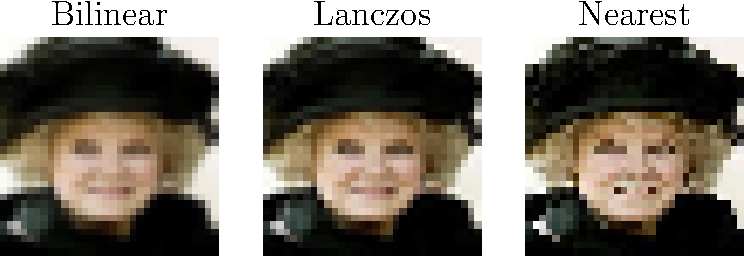
\includegraphics[scale=0.5]{graphics/paper_modelagnostic/celeba_difference_correct_font.pdf}
    \caption{Comparison of different interpolation methods for CelebA dataset.}
    \label{fig_modelagnostic:celeba}
    %  \vspace*{-\baselineskip}
\end{figure}

\begin{table*}[tb]
    %\renewcommand{\thetable}{4}
    \caption{AUROC$\uparrow$ for single-sample OOD detection training on CIFAR10 and testing on CelebA considering all the three interpolations for CelebA.}
    \resizebox{\textwidth}{!}{
        \scriptsize
        \begin{tabular}{ccccccc}
            \toprule
            &\multicolumn{6}{c}{\textsc{CIFAR10 (in) / CelebA (out) ($\dagger$)}}\\
            \cmidrule{2-7}
            & \multicolumn{4}{c}{\textcolor{blue}{\textsc{single statistics}}} & \multicolumn{2}{c}{\textcolor{red}{\textsc{combination}}}\\
            \cmidrule(r){2-5}\cmidrule(l){6-7}
            \textsc{models}  & \textcolor{blue}{\textsc{$\log p(x)$}} & \textcolor{blue}{\textsc{$\|\nabla \log p(x)\|_2$}} & \textcolor{blue}{\textsc{Typicality}} & \textcolor{blue}{\textsc{Score stat}} & \textcolor{red}{\textsc{Fisher's method}} & \textcolor{red}{\textsc{DoSE$_{\textup{KDE}}$}} \\
            \midrule
            \textsc{PixelCNN++} (model1)  &  0.7027 & 0.5856 & 0.5581  & 0.7001 & 0.6450 & 0.6931 \\
            \textsc{PixelCNN++} (model2) & 0.7034  & 0.4298 & 0.5554 & 0.7505 & 0.6879 & 0.7430\\
            \textsc{Glow} (RMSProp)  & 0.5337  & 0.5616 &  0.3926 & 0.6561  & 0.5400 & 0.5866 \\
            \textsc{Glow} (Adam)   & 0.5308  & 0.5820 & 0.3914 & 0.5850  & 0.4818 & 0.5212 \\
            \textsc{HVAE}  &  0.5643 & 0.5214  & 0.4011 & 0.6712 & 0.5483 & 0.5987 \\
            \bottomrule
            & & & & & & \\
            \toprule
            &\multicolumn{6}{c}{\textsc{CIFAR10 (in) / CelebA (out) ($\nparallel$)}}\\
            \cmidrule{2-7}
            & \multicolumn{4}{c}{\textcolor{blue}{\textsc{single statistics}}} & \multicolumn{2}{c}{\textcolor{red}{\textsc{combination}}}\\
            \cmidrule(r){2-5}\cmidrule(l){6-7}
            \textsc{models}  & \textcolor{blue}{\textsc{$\log p(x)$}} & \textcolor{blue}{\textsc{$\|\nabla \log p(x)\|_2$}} & \textcolor{blue}{\textsc{Typicality}} & \textcolor{blue}{\textsc{Score stat}} & \textcolor{red}{\textsc{Fisher's method}} & \textcolor{red}{\textsc{DoSE$_{\textup{KDE}}$}} \\
            \midrule
            \textsc{PixelCNN++} (model1)  &  0.8284  & 0.5035 & 0.7399 & 0.6714  & 0.7477 & 0.7123 \\
            \textsc{PixelCNN++} (model2) & 0.8284 & 0.3530 &   0.7370 & 0.70088 & 0.7631 & 0.7446\\
            \textsc{Glow} (RMSProp)  & 0.7556 & 0.4427 &  0.6222 & 0.7865  & 0.7423 & 0.7632 \\
            \textsc{Glow} (Adam)   & 0.7499 & 0.4800 &  0.6177 &  0.6442  &  0.6460 &  0.6467 \\
            \textsc{HVAE}  & 0.7561 &   0.4097 & 0.6051 &  0.6779 &  0.6775 &  0.6772  \\
            \bottomrule
             & & & & & & \\
            \toprule
            &\multicolumn{6}{c}{\textsc{CIFAR10 (in) / CelebA (out) ($\ddagger$)}}\\
            \cmidrule{2-7}
            & \multicolumn{4}{c}{\textcolor{blue}{\textsc{single statistics}}} & \multicolumn{2}{c}{\textcolor{red}{\textsc{combination}}}\\
            \cmidrule(r){2-5}\cmidrule(l){6-7}
            \textsc{models}  & \textcolor{blue}{\textsc{$\log p(x)$}} & \textcolor{blue}{\textsc{$\|\nabla \log p(x)\|_2$}} & \textcolor{blue}{\textsc{Typicality}} & \textcolor{blue}{\textsc{Score stat}} & \textcolor{red}{\textsc{Fisher's method}} & \textcolor{red}{\textsc{DoSE$_{\textup{KDE}}$}} \\
            \midrule
            \textsc{PixelCNN++} (model1)  & 0.9270  & 0.4196 & 0.8902 &  0.8320 & 0.9287 &  0.8908 \\
            \textsc{PixelCNN++} (model2) & 0.9270 & 0.3065 & 0.8886 & 0.8448 & 0.9339 & 0.9236 \\
            \textsc{Glow} (RMSProp)  & 0.9364 & 0.5345 &  0.8880 & 0.9286  & 0.9390 & 0.9423 \\
            \textsc{Glow} (Adam)   &  0.9322 & 0.5957 & 0.8829  &  0.8350  & 0.9017 &  0.8933 \\
            \textsc{HVAE}  & 0.8964 & 0.3515  & 0.8158 & 0.7952 &  0.8620 &   0.8455 \\
            \bottomrule
            \vspace{-0.2cm}\\
            ($\dagger$) Bilinear interpolation \\
            \hspace{0.06cm}($\nparallel$) Lanczos interpolation \\
            ($\ddagger$) Nearest interpolation\\
        \end{tabular}
        \label{table:celeba}
    }
    % \vspace*{-\baselineskip}
\end{table*}


\section{Comparison with the original DoSE statistics}
As the last experiment, we study how our proposed method with our model agnostic statistic performs against DoSE using the original statistics proposed in \parencite{morningstar_density_2021}. For the VAEs model, they suggested to use the following 5 statistics: the posterior/prior cross-entropy $\text{H}[q_{\phi}( \textbf{z}\mid \textbf{x}), p(\textbf{z})]$, the posterior entropy $\text{H}[q_{\phi}(\textbf{z}\mid \textbf{x})]$, the posterior/prior KL-divergence $\text{D}_{\text{KL}}[q_{\phi}(\textbf{z}\mid \textbf{x}) \mid \mid p(\textbf{z})]$, the posterior expected log-likelihood $\mathbb{E}_{q_{\phi}(\textbf{z}\mid \textbf{x})}[\log q_{\phi}(\textbf{z}\mid \mathbf{x})]$, and the log-likelihood $\log \mathbb{E}_{q_{\phi}(\textbf{z}\mid \textbf{x})} \left[ \frac{p_{\theta}(\textbf{x}, \textbf{z})}{q_{\phi}(\textbf{z}\mid \textbf{x})}\right]$. For DoSE on Glow, instead, they considered three metrics: the log-likelihood $p_{X}(\textbf{x}\mid \theta_n)$ and its two components, i.e.\@ the log-probability of the latent variable $p_{Z}(\textbf{z}\mid \textbf{x}, \theta_n)$ and the log-determinant of the Jacobian $\log | \text{J}_{f}(\textbf{x})|$. 

In this setting, since DoSE is using statistics that are HVAE and Glow specific, it is not model agnostic anymore. Indeed, we cannot use those statistics also for a PixelCNN++ for example or any other DGM. We want also to highlight that the models used in \parencite{morningstar_density_2021} are a bit different from the ones used in this work. For example, they are considering a beta-VAE with only one stochastic layer, while in our case we used a HVAE with 3-stochastic layers. 




\begin{table}[tb]%[15]
    \vspace{-1.3em}
    \caption[Comparison between our method and DoSE using the original statistics]{Comparison between our method and DoSE using the original statistics. In these experiments we considered only Glow trained with Adam.}
        \centering
        \scriptsize
        \begin{tabular}{ccc}
            \toprule
            \textsc{$D_{\text{out}}$}  & \textcolor{red}{\textsc{Our method}} & \textcolor{red}{\textsc{DoSE$_{\textup{orig}}$}} \\
            \midrule
            &\multicolumn{2}{c}{\textsc{GLOW trained on CIFAR10}} \\
            \cmidrule{2-3}
            \textsc{SVHN} & \textbf{0.8613}  &  0.7819  \\
            \textsc{CIFAR100} & \textbf{0.5775} & 0.5700 \\
            \textsc{CelebA} & 0.9017 & \textbf{0.9663}  \\
            %\bottomrule
            %\toprule
            \cmidrule{2-3}
            &\multicolumn{2}{c}{\textsc{GLOW trained on FashionMNIST}} \\
            % \cmidrule{2-3}
            % \textsc{$D_{\text{out}}$}  & \textcolor{red}{\textsc{Our method}} & \textcolor{red}{\textsc{DoSE$_{\textup{orig}}$}} \\
            \cmidrule{2-3}%\midrule
            \textsc{MNIST} & 0.8839 & \textbf{0.9568}   \\
            %\bottomrule
            \midrule%\toprule
            &\multicolumn{2}{c}{\textsc{HVAE trained on FashionMNIST}} \\
            % \cmidrule{2-3}
            % \textsc{$D_{\text{out}}$}  & \textcolor{red}{\textsc{Our method}} & \textcolor{red}{\textsc{DoSE$_{\textup{orig}}$}}  \\
            \cmidrule{2-3}%\midrule
            \textsc{MNIST} & 0.9383 & \textbf{0.9762} \\
            %\bottomrule
            %\toprule
            &\multicolumn{2}{c}{\textsc{HVAE trained on CIFAR10}} \\
            % \cmidrule{2-3}
            % \textsc{$D_{\text{out}}$}  & \textcolor{red}{\textsc{Our method}} & \textcolor{red}{\textsc{DoSE$_{\textup{orig}}$}} \\
            \cmidrule{2-3}%\midrule
            \textsc{SVHN} & 0.8605 & \textbf{0.8823}  \\
            \textsc{CIFAR100} & \textbf{0.5888} & 0.5608  \\
            \textsc{CelebA} & \textbf{0.8620} & 0.8203  \\
            \bottomrule
    \end{tabular}
    \label{table:original_dose}
    % \vspace*{-\baselineskip}
\end{table}


\section{Algorithmic implementation}
A pseudocode describing step-by-step how to implement our method is given in \cref{alg_modelagnostic:algo_description}.

\begin{algorithm}[ht]
%\begin{small}
\begin{algorithmic}
\State \textbf{Input}: Training data $\textbf{X} = (x_1,\ldots,x_m)^T$, validation data $\textbf{X}'$, trained model $p_{\theta}(x)$.\\
\textbf{} \\
\textit{Approximation of the diagonal of the Fisher Information Matrix $I(\theta)$ and average log-likelihood $(1/m)\log p_{\theta}(x_1,\ldots,x_m)$, indicated by $L(\theta)$. We do it in an online fashion.} \\
\textbf{Initialize}  ${I(\theta)} = {0}$ and $L(\theta)=0$ \\
\textbf{For all} $i \in \{1,\ldots ,m\}$: \\
\hspace{1.5em} \textbf{Compute} $\log p_{\theta} ({x}_i)$ \\
\hspace{1.5em} \textbf{Compute} $\nabla_{{\theta}}\log p({x}_i \mid \theta)$ \\
\hspace{1.5em} \textbf{Set}  ${I(\theta)} = \frac{1}{i+1} \cdot (i \cdot {I(\theta)} + (\nabla_{{\theta}}\log p_{\theta}({x}_i))^2$) \\
\hspace{1.5em} \textbf{Set}  $L(\theta) = \frac{1}{i+1} \cdot (i \cdot L(\theta) + \log p_{\theta}({x}_i)$) \\
\textbf{} \\
\textit{Estimation of distributions over the test statistics} \\
\textbf{Sample} $S$ $M'$-sized datasets from $\textbf{X}'$ using bootstrap resampling. \\
\textit{(For single-sample OOD we just cycle through each example, see \cref{sec_modelagnostic:combination_p_values})}\\
\textbf{Initialize}   $T^{\text{typicality}} = [\hspace{0.5mm}]$ and $T^{\text{score}} = [\hspace{0.5mm}]$ \\
\textbf{For every} bootstrapped dataset $\textbf{X}_s' = (x_1, \dots, x_{M'})^T$: \\
\hspace{1.5em} \textbf{Compute} $\frac{1}{m'} \sum_{m'=1}^{M'}\log p_{\theta}({x}_{m'})$ \\
\hspace{1.5em} \textbf{Compute} $\frac{1}{m'} \sum_{m'=1}^{M'}\nabla_{{\theta}}\log p_{\theta}({x}_{m'})$ \\
\hspace{1.5em} \textbf{Compute} MMD Typicality for ${x}_{m'}$ by $\left\| \frac{1}{m'} \sum_{m'=1}^{M'}\log p_\theta ({x}_{m'}) - L(\theta) \right\|_2$ and add it to $T^{\text{typicality}}$\\
\hspace{1.5em} \textbf{Compute} Score statistic for ${x}_{m'}$ by $\left\|{I(\theta)}^{-1/2} \frac{1}{m'} \sum_{m'=1}^{M'}\nabla \log p_\theta ({x}_{m'})\right\|_2$ and add it to $T^{\text{score}}$\\
\textbf{Return} Two vectors of size $S$ containing the two statistics for $T^{\text{typicality}}$ and $T^{\text{score}}$  \\
\textbf{} \\
\textbf{Compute} $\hat{F}^{\text{typicality}}$ and $\hat{F}^{\text{score}}$, the two empirical CDFs, from $T^{\text{typicality}}$ and $T^{\text{score}}$. For example, we used \texttt{statsmodels} library \parencite{seabold_statsmodels_2010}. \\
\textbf{} \\  
%\textit{For any test sample} \\
\textbf{Given} a test set $\tilde{x}_1, \dots, \tilde{x}_n$:\\
\textit{($n=1$ corresponds to perform single-sample OOD detection)} \\ 
\hspace{1.5em} \textbf{Compute} $\frac{1}{n} \sum_{i=1}^{n}\log p_{\theta}(\tilde{{x}}_i)$ and $\frac{1}{n} \sum_{i=1}^{n}\nabla_{{\theta}}\log p_{\theta}(\tilde{{x}}_i)$ \\
\hspace{1.5em} \textbf{Compute} MMD Typicality $\tilde{t}$ and Score statistic $\tilde{s}$ \\
\hspace{1.5em} \textbf{Compute} $p$-values $p_{T} = 1 - \hat{F}^{\text{typicality}}(\hat{t})$ and $p_{S} = 1 - \hat{F}^{\text{score}}(\tilde{s})$ \\
\hspace{1.5em} \textbf{Combine} the two $p$-values using Fisher's method \cref{eq_modelagnostic:Fisher_method}
\end{algorithmic}
\caption{Computing $p$-values for OOD detection using a trained generative model.}
\label{alg_modelagnostic:algo_description}
%\end{small}
\end{algorithm}

}